\chapter{Návrh a implementace}\label{navrh}
V této kapitole budou popsány změny návrhu programu, které se skládají z navržených změn podle požadavku frontendového týmu a návrhu chybějící funkcionality. Také bude popsána implementace změn návrhu a chybějící funkcionality. A také, bude popsán návrh a následní implementace funkcí, které jsou zaměřené na zlepšení kvality výsledného softwaru.

Při úpravách současného návrhu byl udělán velký počet změn různé významnosti. V této kapitole budou uvedeny klíčové změny. Při implementaci návrhu autorovi pomohlo přečteni doporučené literatury.\cite{pro-spring-boot-2}

\section{Úpravy podle požadavků frontendového týmu}\label{navrh:upravy}
    V této sekci budou popsány navržené změny podle požadavků frontendového týmu a jejích následná implementace.
    
    \subsection{Interval}\label{navrh:upravy:interval}
        \begin{figure}\centering
	        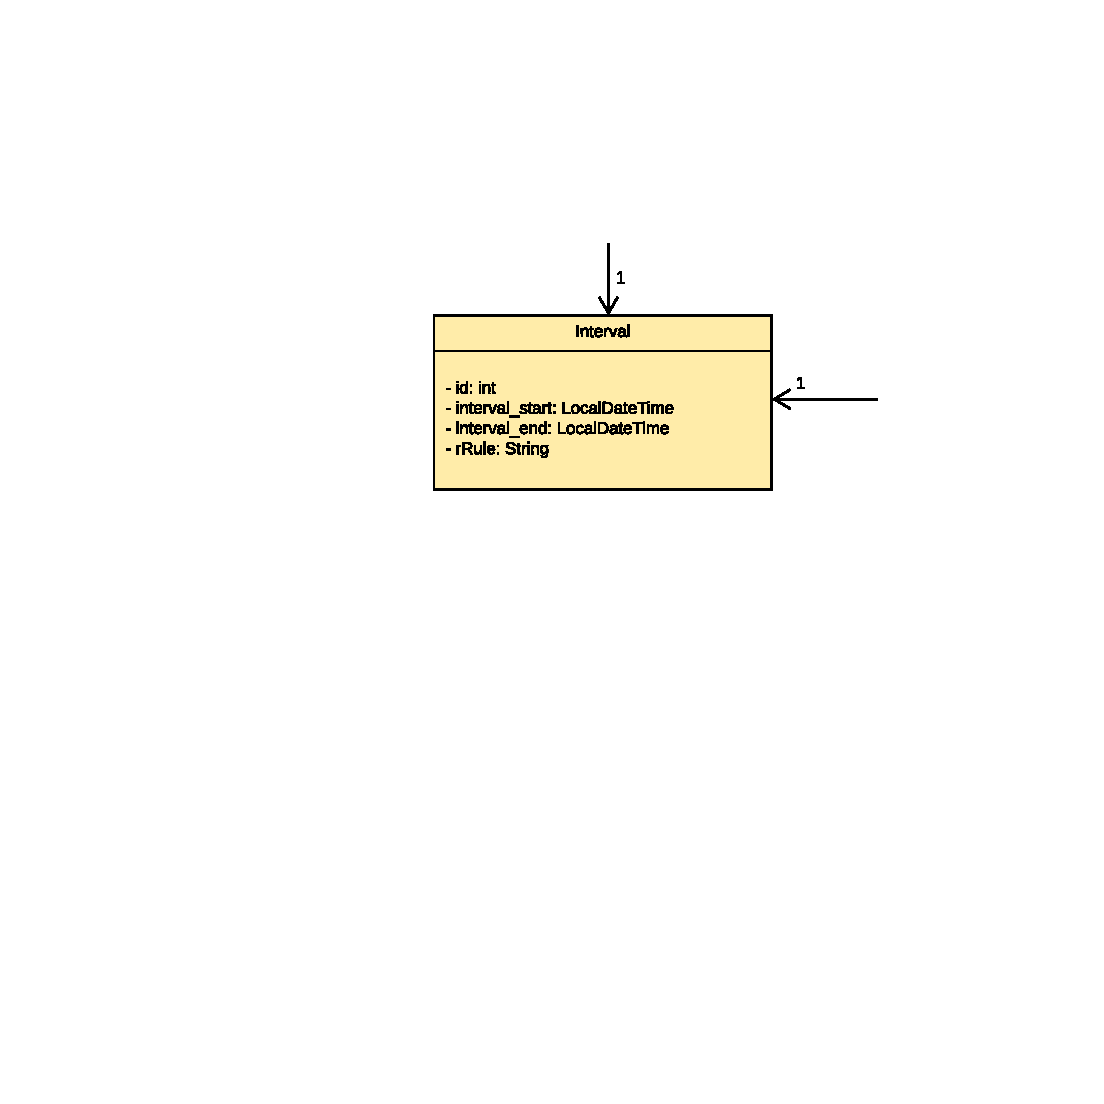
\includegraphics[width=0.7\textwidth]{pdfs/Interval2}
	        \caption[Nový návrh entity \texttt{Interval}]{Nový návrh entity \texttt{Interval}}\label{image:Interval2}
        \end{figure}
        \begin{figure}\centering
	        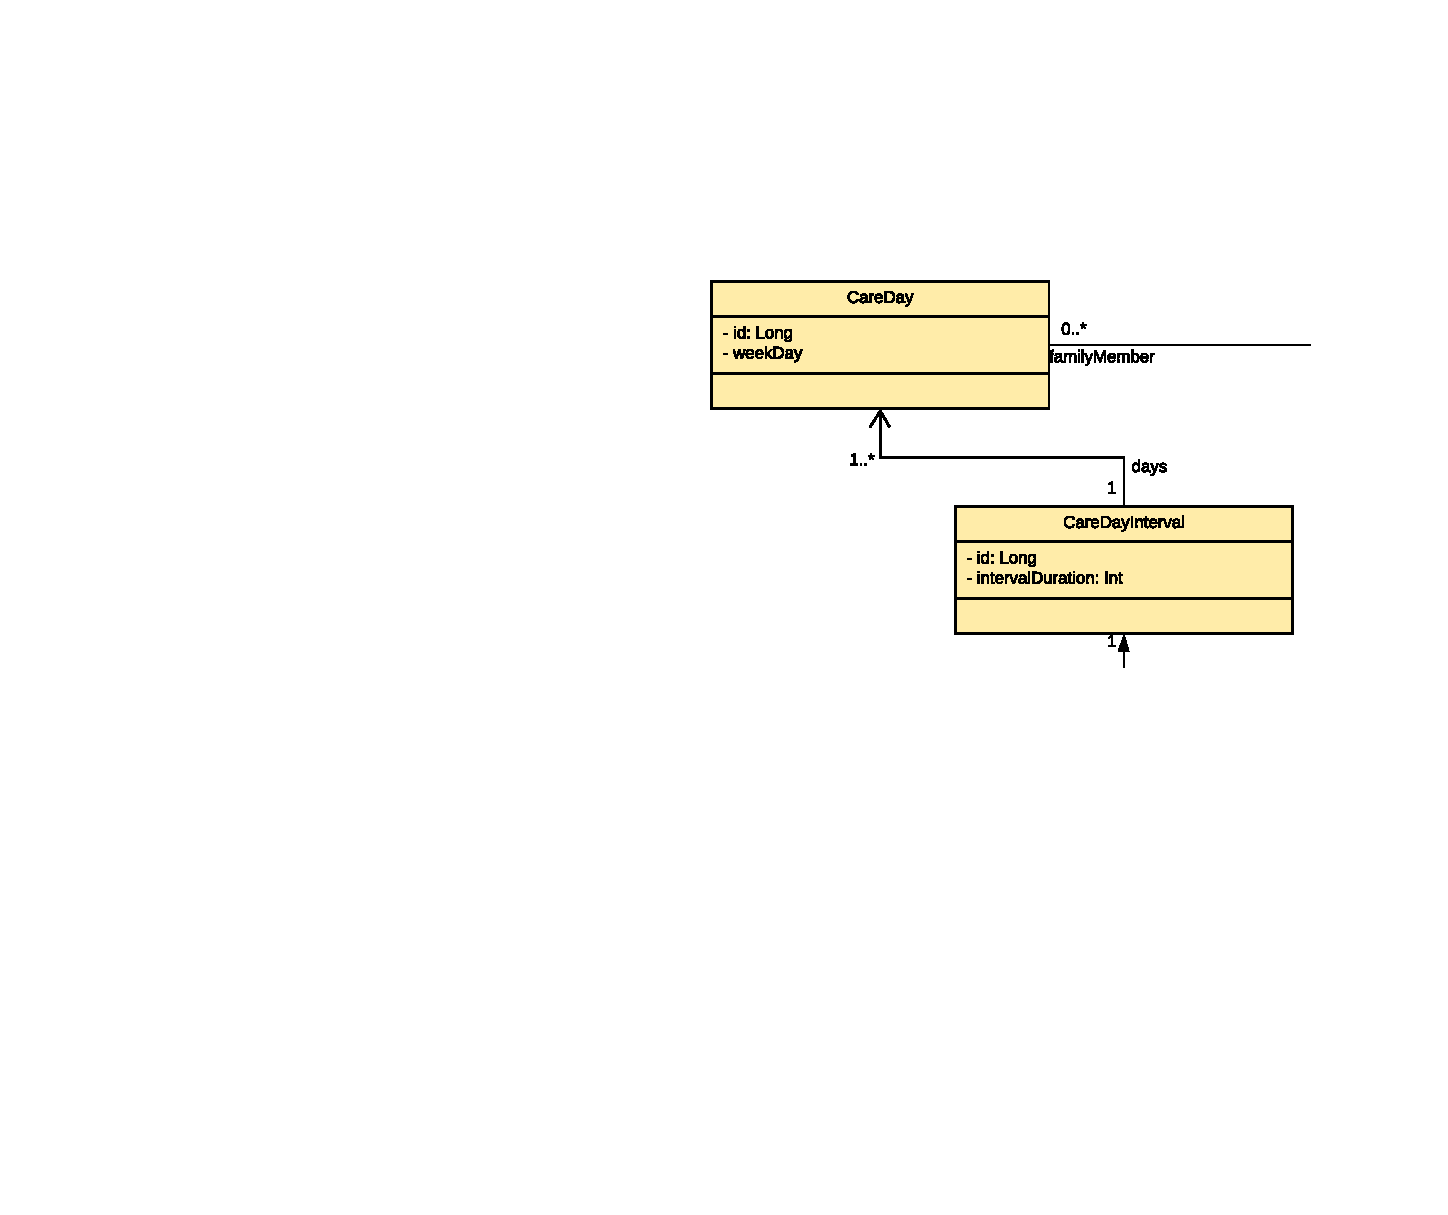
\includegraphics[width=0.8\textwidth]{pdfs/CareDayInterval}
	        \caption[Návrh entity \texttt{CareDayInterval}]{Návrh entity \texttt{CareDayInterval}}\label{image:careDayInterval}
        \end{figure}
        První změnou je nový návrh entity \verb|Interval|. Původní návrh nevyhovoval svojí složitostí a zároveň jenom částečným pokrytím možných případů využití (viz~obrázek~\ref{image:Interval1}). Entita řešila několik samostatných problémů najednou: pravidla pečovatelských dnů rodičů a klasické intervaly definující pravidla opakování nebo jednorázovou událost. Proto entita \verb|Interval| byla rozdělena do dvou samostatných částí.
        První část se zabývá pravidly pro pečovatelské dny rodičů (viz obrázek \ref{image:Interval2}). Pravidlo je reprezentováno intervalem, který se opakuje, a skládá se ze seznamu jednotlivých pečovatelských dnů. Každý pečovatelský den je navázán na konkretního rodiče, který je zodpovědný za dítě v tento den. Použití tohoto typu intervalu bude popsané v sekci \ref{navrh:upravy:caredays}. Ostatní případy použití intervalů nevyžadují, ani specifické atributy, ani specifický rozsah možných pravidel, proto ostatní případy použití řeší stejná entita -- \verb|Interval| -- (viz obrázek \ref{image:Interval2}).
        
        % První část reprezentuje (viz obrázek \ref{image:Interval2}) úplně nahrazuje původní entitu. Druhou entitou je \texttt{CareDayInterval} (viz obrázek \ref{image:careDayInterval}), která reprezentuje časové rozmezí pečovatelských dnů.
    
        Nový návrh entity \verb|Interval| je kompilovaný, proto je potřeba podrobně popsat použitou architekturu. Nový návrh je postaven na jiném principu, kde časové rozmezí může být reprezentované dvěma způsoby. Oba dva způsoby vyžadují uvedení začátku intervalu. Tento parametr je povinný. První způsob, kromě začátku intervalu, vyžaduje i konec intervalu. Takovým způsobem můžeme definovat jednorázový interval po sobě jdoucích dnů. Druhý způsob vyžaduje zadání pravidla opakování. Takhle můžeme definovat stejný interval, ale mnohem složitějším způsobem. Na druhou stranu, pomocí takového pravidla můžeme definovat libovolně složitý interval. 
        Například, zmíněný v sekci \ref{analyza:pozadavky:interval}, interval, který se bude opakovat každý poslední den měsíce. Výsledný návrh sestavení intervalu vyžaduje aby, buď byl zadán jenom konec intervalu, nebo bylo zadáno jenem pravidlo opakování. V případě, že tyto dva parametry budou zadány najednou, server vyhodí chybu a zastaví vytvoření nesprávného intervalu.
    
        Pravidlo opakování je reprezentováno pomocí textového řetězce, který má být zadán podle standardu {RFC 5545}\cite{recurrence-rule}. Pro pohodlné testování byl navržen a implementován {interní DSL jazyk}\footnote{DSL jazyk využívající obecný programovací jazyk}, který bude popsán v sekci \ref{navrh:zmeny:dsl}.
        
    \subsection{Alimenty}\label{navrh:upravy:alimenty}
        Druhou důležitou úpravou současného návrhu je změna entity \verb|Alimony| a spravování instancí této třídy.
    
        \subsubsection{Úprava entity}
            Za účelem zvýšení samostatnosti instancí entity \verb|Alimony| byla přidána závislost na entitu \verb|Family|. Také byl přidán atribut \verb|value|, který se kopíruje z entity \verb|AlimonySetting|. Příčinou přidání tohoto atributu je možnost aktualizování nastavení alimentů, což působí zneplatnění již existujících instancí alimentů. V případě, že rodiče změní hodnotu v nastaveních alimentů, ztratí se možnost zjistit hodnoty alimentů, které byly vytvořeny do změny.
            
        \subsubsection{Spravování alimentů} 
            V této sekci bude popsán návrh třídy, která se věnuje vytváření alimentů.
        
            \begin{figure}
                \begin{minted}[frame=lines,
        framesep=2mm,
        baselinestretch=1.2,
        fontsize=\footnotesize,
        linenos]{java}
/**
*  Method generating Alimony instances based 
*   on AlimonySettings(enabled) from DB.
*
*  Scheduling is configured by the cron expression,
*  that you need to configure in application-{profile}.properties 
*   (scheduled.alimonyFactory.cronExpression).
*/
@Scheduled(cron = "\${scheduled.alimonyFactory.cronExpression}")
fun createAlimonyForEachAlimonySetting() {
    logger.info("Started scheduled alimony creation process;")
    val alimony = alimonySettingRepository
                        .findAllByEnabledTrue()
                        .map { it.createAlimony() }
    if (alimony.isNotEmpty()) {
        alimonyRepository.saveAll(alimony)
    } else {
        logger.debug(
            "AlimonyFactory didn't find any AlimonySetting to work with;"
            )
    }
}
                \end{minted}
                \caption{Ukázka metody vytvářející instance alimentů} 
                \label{code:create-alimony}
            \end{figure}
            Všechny instance alimentů je potřeba vytvářet pravidelně. Proto vytváření bylo objednáno do jednoho procesu, který je stejný pro všechny instance. Proces vytváření alimentů zajišťuje specifická metoda, která se nachází ve třídě \verb|AlimonyFactory| (viz obrázek \ref{code:create-alimony}). Metoda vyhledává všechny aktivní instance \verb|AlimonySetting| a pro každou vytvoří instanci entity \verb|Alimony|. 
            
            % Proces vytváření alimentů je nastavitelný pomoci proměnných prostředí příslušného profilu.
            \begin{figure}
                \begin{minted}[frame=lines,
        framesep=2mm,
        baselinestretch=1.2,
        fontsize=\footnotesize,
        linenos]{yaml}
\# Cron expression: at 01:01 AM on the 1st day of every month
scheduled.alimonyFactory.cronExpression=0 1 1 1 * ?
                \end{minted}
                \caption{Ukázka konfigurace \texttt{cron} výrazu pro plánování vytváření alimentů} 
                \label{code:cron-expression}
            \end{figure}
            Vytvářeni alimentů má být pravidelné a nemusí vyžadovat účast člověka. Proto byla využita funkcionalita frameworku Spring, která poskytuje možnost plánování automatického spouštěni.\cite{spring-scheduling} Anotace \verb|@Scheduled| vytváří s dáne metody komponentu, která se vykonává podle uvedeného pravidla. Existuje několik podporovaných typu pravidel. 
            Například nastavení intervalu mezi nastartováními nebo mezi ukončeními. Ale pro plánovaní vytváření alimentů je potřeba nastavit konkretní den měsíce nebo roku, který se bude opakovat. Proto bylo zvoleno \verb|cron| pravidlo, které je také podporováno anotací.\cite{cron-expression} Tento výraz je textovou řádkou, která se skládá z čísel oddělených čárou, reprezentujících čas spouštění.
            Toto pravidlo nebylo zadáno přímo do kódu. Pro přidání možnosti pohodlné konfigurace pravidla byla definována proměnná prostředí, která se nachází v konfiguračním souboru příslušného profilu (viz obrázek \ref{code:cron-expression}). Implementace byla provedena podle návody z knihy\cite{sbr:spring-task-scheduling}. Podrobněji profily budou popsány v sekci \ref{navrh:profily}.
         
            % Anotace \verb|Scheduled|, která zapíná plánování pro konkretní metodu, vyžaduje \texttt{cron} výraz. Tento výraz je textovou řádkou, která se skládá z čísel oddělených čárou, reprezentujících čas spouštění metod\cite{cron-expression}. Implementace byla provedena podle návody z knihy\cite{sbr:spring-task-scheduling}.
            % Pro pohodlnou konfiguraci času spouštěni metody, \texttt{cron} výraz byl přesunut do souboru \texttt{application-{profile}.properties}, kde \texttt{profile} je aktuální profilem serveru. Podrobněji návrh profilu bude popsán v sekci \ref{navrh:profily}. Pro zadání \texttt{cron} výrazu je potřeba definovat \texttt{property} \texttt{scheduled.alimonyFactory.cronExpression} (viz obrázek \ref{code:cron-expression}).
            \begin{figure}
                \begin{minted}[frame=lines,
        framesep=2mm,
        baselinestretch=1.2,
        fontsize=\footnotesize,
        linenos]{yaml}
scheduled.alimonyFactory=true
                \end{minted}
                \caption{Ukázka proměnné prostředí zapínající \texttt{AlimonyFactory}} 
                \label{code:alimony-factory-true}
            \end{figure}
            Byla přidána možnost měnit čas spouštění metody pomocí konfiguračního souboru, ale také bychom potřebovali mít možnost vypnout tuto metodu. Například, pro robustní testování. Proto byla přidána třída, která vytváří instanci tříd, obsahující automaticky spustitelné metody. Třída je definována jako komponenta frameworku Spring a každá její metoda je určena pro vytváření instancí jiných tříd podle předem definované podmínky.
            V případě, že podmínka má hodnotu \verb|false|, příslušná komponenta se nevytváří.
            Pro vytváření třídy \verb|AlimonyFactory| byla definována podmínka, která ověřuje jestli proměnná \verb|scheduled.alimonyFactory| je nastavená na hodnotu \verb|true| (viz obrázek \ref{code:alimony-factory-true}). V případě, že tato proměnná nebyla definována pro aktuální profil aplikace, proměnná se automaticky nastaví na hodnotu \verb|false| a instance třídy \verb|AlimonyFactory| nebude vytvořena.
            % podle \texttt{property} konfiguračního souboru. V případě, že nutné \texttt{property} nebyly definovány aplikace se neukončí běh a nastaví tyto \texttt{property} na implicitní hodnoty. Pro zapínaní běhu metody vytvářející alimenty je potřeba definovat \texttt{property} \texttt{scheduled.alimonyFactory} a nastavit na hodnotu \texttt{true} (viz obrázek \ref{code:alimony-factory-true}).
        
    \subsection{Pečovatelské dny}\label{navrh:upravy:caredays} % PECOVATELSKE DNY
        \begin{figure}\centering
	       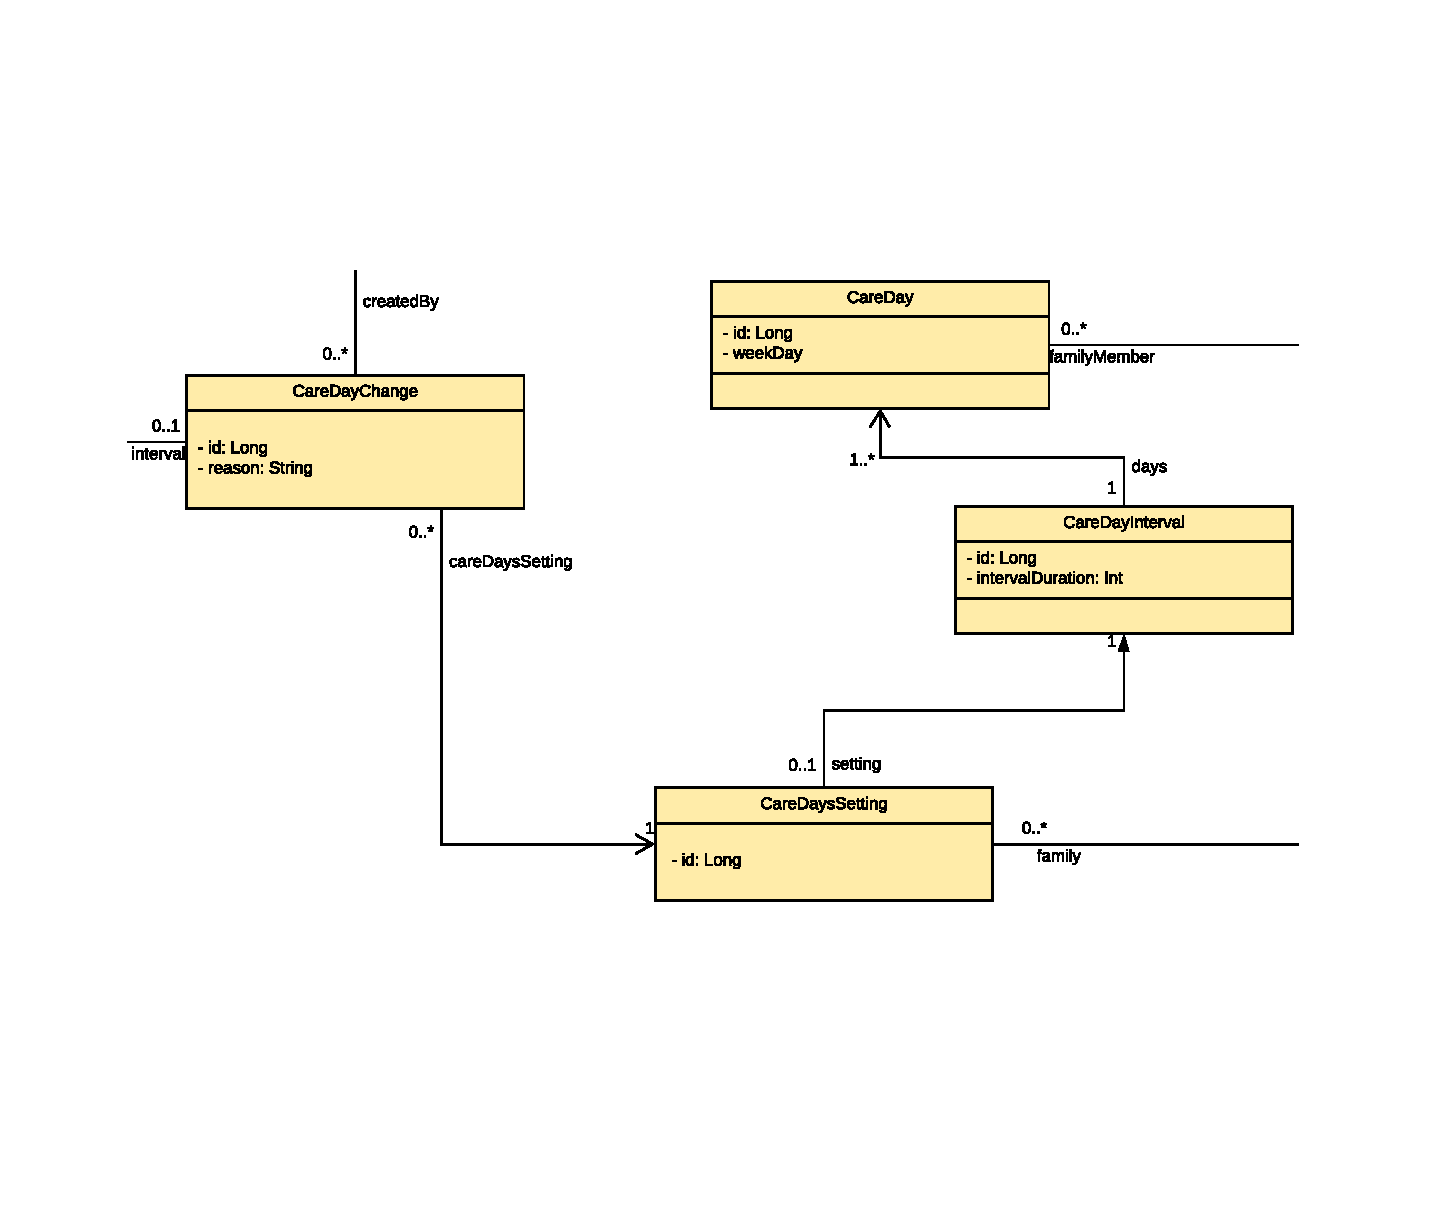
\includegraphics[width=1.0\textwidth]{pdfs/CareDays2}
	       \caption[Nový návrh pečovatelských dnů]{Nový návrh pečovatelských dnů}\label{image:caredays2}
        \end{figure}
        V předchozím návrhu implementace dlouhodobé nastavení pečovatelských dnů pro rodiče a jednorázové změny byly reprezentované pomocí jedné entity (viz obrázek \ref{image:caredays1}). Problém je právě ve sjednocení několika problému do jednoho. Proto bylo rozhodnuto rozdělit řešení do dvou částí. Výsledný návrh se skládá ze čtyř entit (viz obrázek \ref{image:caredays2}):
        \begin{itemize}
            \item \texttt{CareDaysSetting}, reprezentující dlouhodobé nastavení pečovatelských dnů;
            \item \texttt{CareDayInterval}, reprezentující interval pečovatelských dnů pro dlouhodobé nastavení;
            \item \texttt{CareDay}, reprezentující jeden pečovatelský den pro dlouhodobé nastavení;
            \item \texttt{CareDayChange}, reprezentující změnu pečovatelských dnů.
        \end{itemize}
        Dlouhodobé nastavení pečovatelský dnů rodičů již byly zmíněné v sekci \ref{navrh:upravy:interval}. Nastavení se skládají z po sobě jdoucích dnů, kde každý den má odkaz na rodiče který má v péče dítě v tento den. Interval je uchováván v entitě \verb|CareDaysSetting|, která reprezentuje nastavení pečovatelských dnů rodičů pro konkretní rodinu. Tyto nastavení definují implicitní nastavení pečovatelských dnů, podle kterých se vyplní kalendář rodiny.
        
        Změny pečovatelských dnů jsou reprezentovány entitou \verb|CareDayChange|. Změna může být, jak jednorázová, tak i dlouhodobá. Interval změny nebo pravidlo opakování změny je reprezentován pomocí entity \verb|Interval|. Každá změna se vztahuje ke konkretnímu členu rodiny a instanci nastavení pečovatelských dnů příslušné rodiny.
        % Dlouhodobá nastavení jsou reprezentovány seznamem pečovatelských dnů, kde každý den má odkaz na člena rodiny, který má v tento den peče o dítě. Jeden \texttt{CareDayInterval} obsahuje seznám takových pečovatelských dnů, ale nereprezentuje nastavení. Za účelem pohodlné modifikovatelností, \texttt{CareDayInterval} je jenom pomocnou entitou, kterou udržuje entita \texttt{CareDaysSetting}, reprezentující dlouhodobé nastavení pečovatelských dnů. Tudíž, uživatel má možnost změnit interval pečovatelských dnů tím, že nahradí jiným záznamem, a současně bude vytvořena kopie tohoto záznamu v historii (viz sekci \ref{navrh:testovani}).
        
    \subsection{Oznámení}\label{navrh:upravy:notification}
        \begin{figure}\centering
	       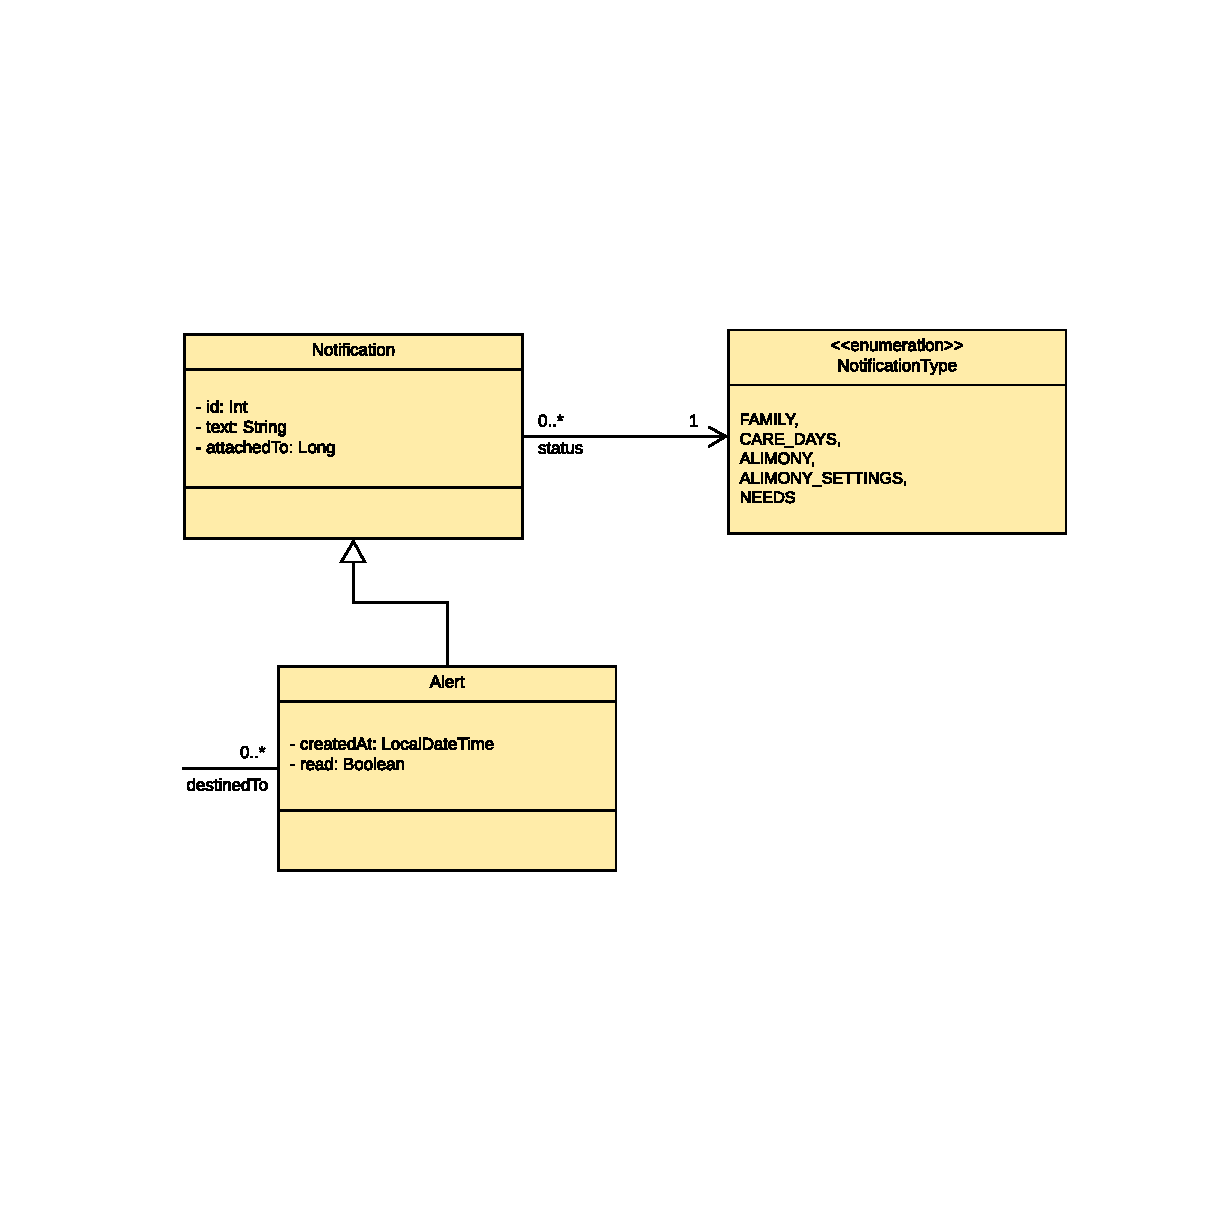
\includegraphics[width=0.8\textwidth]{pdfs/Notification2}
	       \caption[Nový návrh oznámení]{Nový návrh oznámený entity \texttt{Notification} a navazujících se na ně entit}\label{image:notification2}
        \end{figure}
        Předchozí návrh oznámení nebyl vhodný pro frontendovou část aplikace. Oznámení byly určeny jenom pro konkretní případ využití -- oznámení o požadavku na změnu. Také oznámení byly navrženy obecně a neměly konkretní typ. Tudíž oznámení elektronické pošty a upozornění v telefonu byly reprezentovány pomocí stejné entity.
        
        Předchozí abstraktní entita byla určena pro definování základních údajů. Zděděna entita definovala důležitost tohoto oznámení pro konkretního uživatel a uživatele samotného. Bylo rozhodnuto zachránit abstraktní návrh entity \verb|Notification|, ale změnit jeho účel. Abstraktní entita bude obsahovat základní údaje pro všechny typy oznámení. Zděděné entitu budou reprezentovat konkretní typ oznámení.
        Současná implementace frontendové částí aplikace vyžaduje přizpůsobení entity oznámením v rámci Android aplikace. Proto byla přidaná entita \verb|Alert| (viz obrázek \ref{image:notification2}), která dědí základní údaje od entity \verb|Notification|. Pro zaručení konkretizace příčiny vytvoření oznámení byl přidán odkaz na událost do abstraktní entity a také typ této události. Typ oznámení je reprezentován pomoci entity výčtového typu -- \verb|AlertCause|. 
        Každá instance entity \verb|Alert| obsahuje atribut \verb|read| označující jestli je oznámení přečteno uživatelem. Pro zaručení kvalitního návrhu API, byla přidána možnost přečtení všech upozornění najednou. Přečtení upozornění je reprezentováno pomocí přidání atributu \verb|read| hodnoty \verb|true|.
        
        Pro dosažení kvalitnějšího výsledku také byla odstraněna závislost na entitu \verb|Comment|, protože výsledný návrh oznámení nepotřebuje přidávání komentáře. Také byl přidán atribut \verb|text|, který je nutným pro uváděni podrobnějšího popisu oznámení.
            
\section{Navržené změny}
    V této sekci budou popsány navržené autorem této práci změny zaměřené na vylepšení výsledné aplikace.
    
    \subsection{Interní DSL jazyk}\label{navrh:zmeny:dsl}
        % TODO popsat podrobneji
        \begin{figure} % [H] TODO
            \begin{minted}[frame=lines,
        framesep=2mm,
        baselinestretch=1.2,
        fontsize=\footnotesize,
        linenos]{java}
/**
* Valid Interval with recurrence rule.
*/
private val validInterval = Interval(
        id = 1,
        interval_start = creationTime,
        interval_end = null,
        rRule = rule(frequency = Frequency.WEEKLY, count = 10) {
            byDays {
                and(DayOfWeek.MONDAY)
                and(DayOfWeek.WEDNESDAY)
                and(DayOfWeek.SUNDAY)
            }
        }
)
            \end{minted}
            \caption{Ukázka instance entity \texttt{Interval} s pravidlem opakování} 
            \label{code:valid-interval}
        \end{figure}
        Pro pohodlné testování entit závisících na entitě \verb|Interval| byl implementován interní DSL\footnote{\textit{domain specific language}} jazyk, poskytující možnost vytvořit pravidlo opakovaní. Na obrázku \ref{code:valid-interval} je zobrazen příklad intervalu, který má pravidlo opakování vytvořené pomoci DSL jazyku. Příklad je převzat ze současné implementace testování.

    \subsection{Album}
        Libovolný člen rodiny může mít několik vlastních albumu, které potřebuje rozlišovat mezi sebou. Předchozí návrh entity \verb|Album| neposkytoval možnost přidání názvu, proto do entity byl přidán příslušný atribut.
        
    \subsection{Konverter}
        V sekci \ref{analyza:soucasnaImplementace} již bylo zmíněno, že pro implementaci serveru byla zvolena třívrstvá architektura. Doménová vrstva komunikuje s datovou vrstvou pomocí tříd reprezentujících entity databáze, ale s aplikační vrstvou tato komunikace se provádí pomoci DTO. Konverze mezi entitou a dto se provádí v této vrstvě. Za konverzí z entity na dto odpovídá třída entity. Za konverzi z dto na entitu odpovídá třída dto.
        Takový postup těsně provazuje entitu s příslušnou třídou dto, tenhle problém se také nazývá \textit{tight coupling}. Zavedení konvertorů je přizváno zmenšit takovou závislost. Každý konvertor obsahuje metodu konvertující entitu na příslušné dto a metodu konvertující dto na příslušnou entitu. Takový postup umožňuje odstranit stejné metody z příslušných tříd, což zvětšuje modularitu návrhu. 
        Pak je možné snadno přidat jiné DTO reprezentující stejnou entitu bez úprav entity samotné, a naopak.
        
        
        \begin{figure} % [H] TODO
            \begin{minted}[frame=lines,
        framesep=2mm,
        baselinestretch=1.2,
        fontsize=\footnotesize,
        linenos]{java}
internal interface InterfaceConverter<E : InterfaceEntity, D : InterfaceDTO> {

    fun convertToEntity(dto: D): E

    fun convertToDTO(entity: E): D

}
            \end{minted}
            \caption{Ukázka rozhraní \texttt{InterfaceConverter}} 
            \label{code:interface-converterl}
        \end{figure}
        Za účelem dosažení kvalitnějšího výsledku a zrychlení implementaci bylo zavedeno rozhraní definující implicitní metody pro každý konvertor (viz obrázek \ref{code:interface-converterl}). Rozhraní také potřebuje zadání typu entity a dto, které mají být podtřídami \verb|InterfaceEntity| a \verb|InterfaceDTO|. 
        
    \subsection{Našeptavač pro výjimky}
        Našeptavač pro výjimky již byl zmíněn v sekci \ref{analyza:implementace:tridy}. Tato komponenta byla rozšířena o typ výjimky označující, že dto nebyl správně serializován kvůli nedostatku potřebných atributů. Příkladem může být překlep v názvu povinného atributu. Také návratová zpráva byla rozšířená o textový název chyby a časové razítko. Výslednou konfiguraci našeptavače najděte v příloze \ref{dodatek:excpetion-handler2}.
        
    \subsection{Aplikační vrstva}
        V předchozí implementaci byl použit POST požadavek, jak pro vytváření, tak i pro aktualizování. Požadavky se rozlišují mezi sebou přítomností identifikátoru. Pokud ID je nastaven na \verb|null| vytvoří se nový záznam v databází. V opačném případě, server se pokusí najít a aktualizovat záznam.
        
        
        Nový návrh aplikační vrstvy podporuje POST a PUT požadavky. POST požadavek je určen pro vytvoření nového záznamu a vyžaduje aby atribut \verb|id| v dto byl nastaven na hodnotu \verb|null|. PUT požadavek je určen pro aktualizaci záznamu a vyžaduje aby atribut \verb|id| v dto byl nastaven na číslo.
        
        
        Jeden uživatel může být současně členem několika různých rodin. Serverový backend nemůže předem vědět ve které rodině se aktuálně uživatel nachází. Proto do API byly přidány požadavky, které vyžadují zadání identifikátoru konkretní rodiny. Na základě tohoto identifikátoru se filtrují záznamy, které obdrží uživatel. Požadavky nevyžadující identifikátor rodiny nebyly odstraněny, protože všechny požadavky procházejí proces filtraci. Následně konečný uživatel obdrží jenom záznamy, které jsou pro něho dostupné.
        
        
        Dokumentace aplikační vrstvy také byla rozšířena o návratové statusy pro každou metodu. Všechny parametry metod jsou získány z požadavků, proto byly také přidány podrobné popisy parametrů metod. 
        
    \subsection{Doménová vrstva}%prejmenovat na ceskou verzi
        Nový návrh aplikační vrstvy rozděluje proces vytváření nových záznamů a proces aktualizaci již existujících záznamů. Proto tento proces byl rozdělen do dvou separátních procesu i v doménové vrstvě.
        
        
        Proces filtrování záznamu podle aktuálně přihlášeného uživatele se provádí na datově vrstvě. Doménová vrstva jenom používá specifické metody datové vrstvy obsahující filtraci. V případě, že požadována data se nepatří konkretnímu uživateli, ale celé rodině, provádí se ověření jestli aktuálně přihlášený uživatel patří do této rodiny,
        
    \subsection{Datová vrstva}
        V předchozí implementaci datové vrstvy byly použity implicitní metody, které poskytuje framework Spring Data. V současné implementace byly přidány vlastní metody s použitím nástroje pro vytváření metod dotazování (\textit{query methods}). Přidané metody jsou zavedeny za účelem filtrování záznamu, které obdrží uživatel. Filtrování se provádí na základě údajů o aktuálně přihlášeném uživateli. 
        V případě, že požadované záznamy nepatří konkretnímu uživateli, ale patří cele rodině, ověřuje se jestli aktuálně přihlášený uživatel patří do této rodiny.
    
    \subsection{Implementace historie změn}
        Důležitou částí aplikace je zaznamenání změn udělaných uživatelem. Úpravou je změna záznamu entity, kterou uživatel s rolí \enquote{ROLE\_USER} může upravit. Takovou roli má libovolný přihlášený do systému uživatel. Aktivita \texttt{root}\footnote{uživatel s rolí \enquote{ROLE\_ROOT}} uživatele není uvažována, protože tento uživatel není přítomný v rámci profilu pro produkci. Příkladem takové změny může být změna nastavení alimentů nebo označení oznámení jako přečtené.
    
        \begin{figure}\centering
	        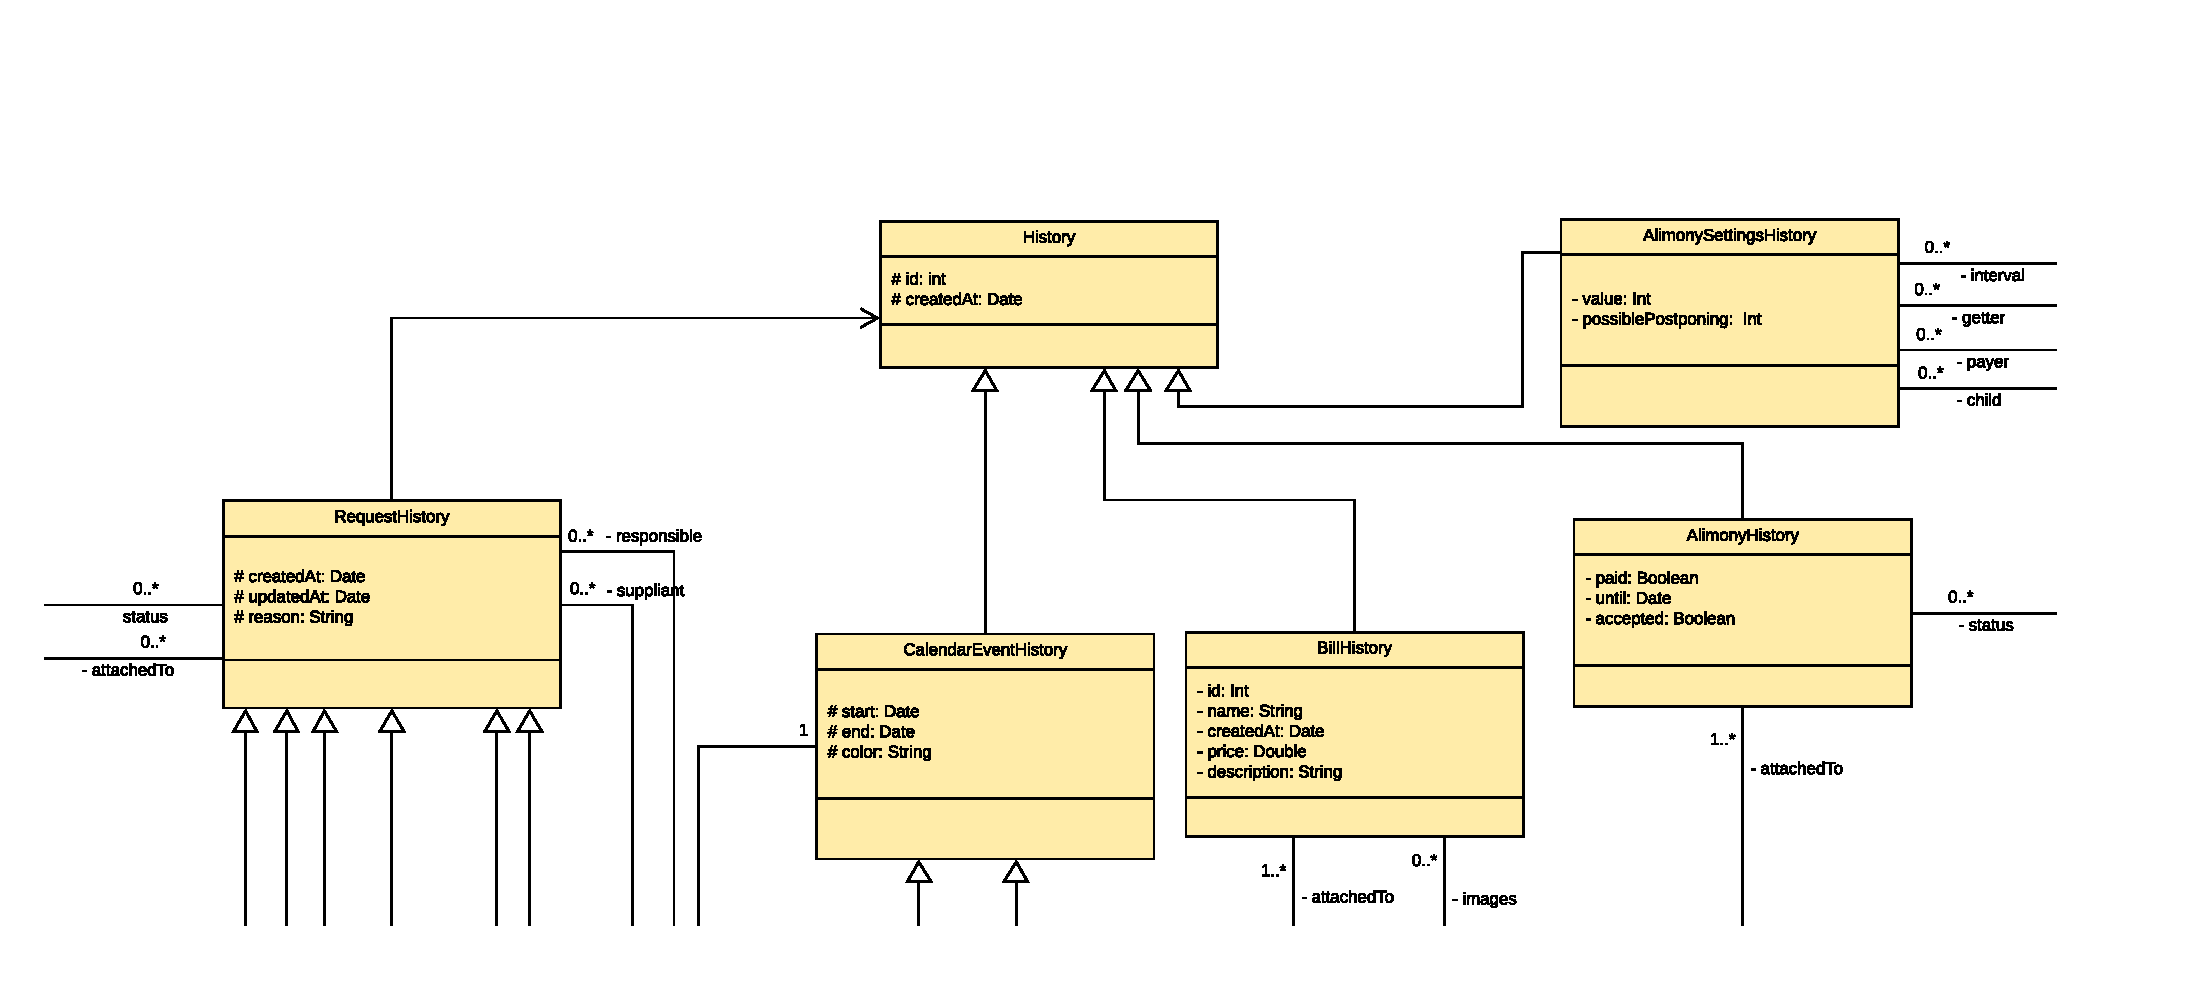
\includegraphics[width=1.0\textwidth]{pdfs/History1}
	        \caption[Předchozí návrh entity \texttt{History}]{Předchozí návrh entity \texttt{History} podle doménového modelu z předmětu BI-SP2}\label{image:History1}
        \end{figure}
        Historie změn ještě nebyly implementovány, ale návrh již existoval a hlavní myšlenka se zůstává úplně stejnou. Záznam historie kopíruje všechny atributy entity a přidává čas vytvoření záznamu a vlastní identifikátor\footnote{identifikátor v rámci databáze}. Entita \verb|History| je abstraktní třídou, neboli generalizace v případě návrhu v doménovém modelu. Jednotlivé entity, které jsou zděděné od této entity, reprezentují historie příslušných entit (viz obrázek \ref{image:History1}). 
    
        \begin{figure}\centering
	        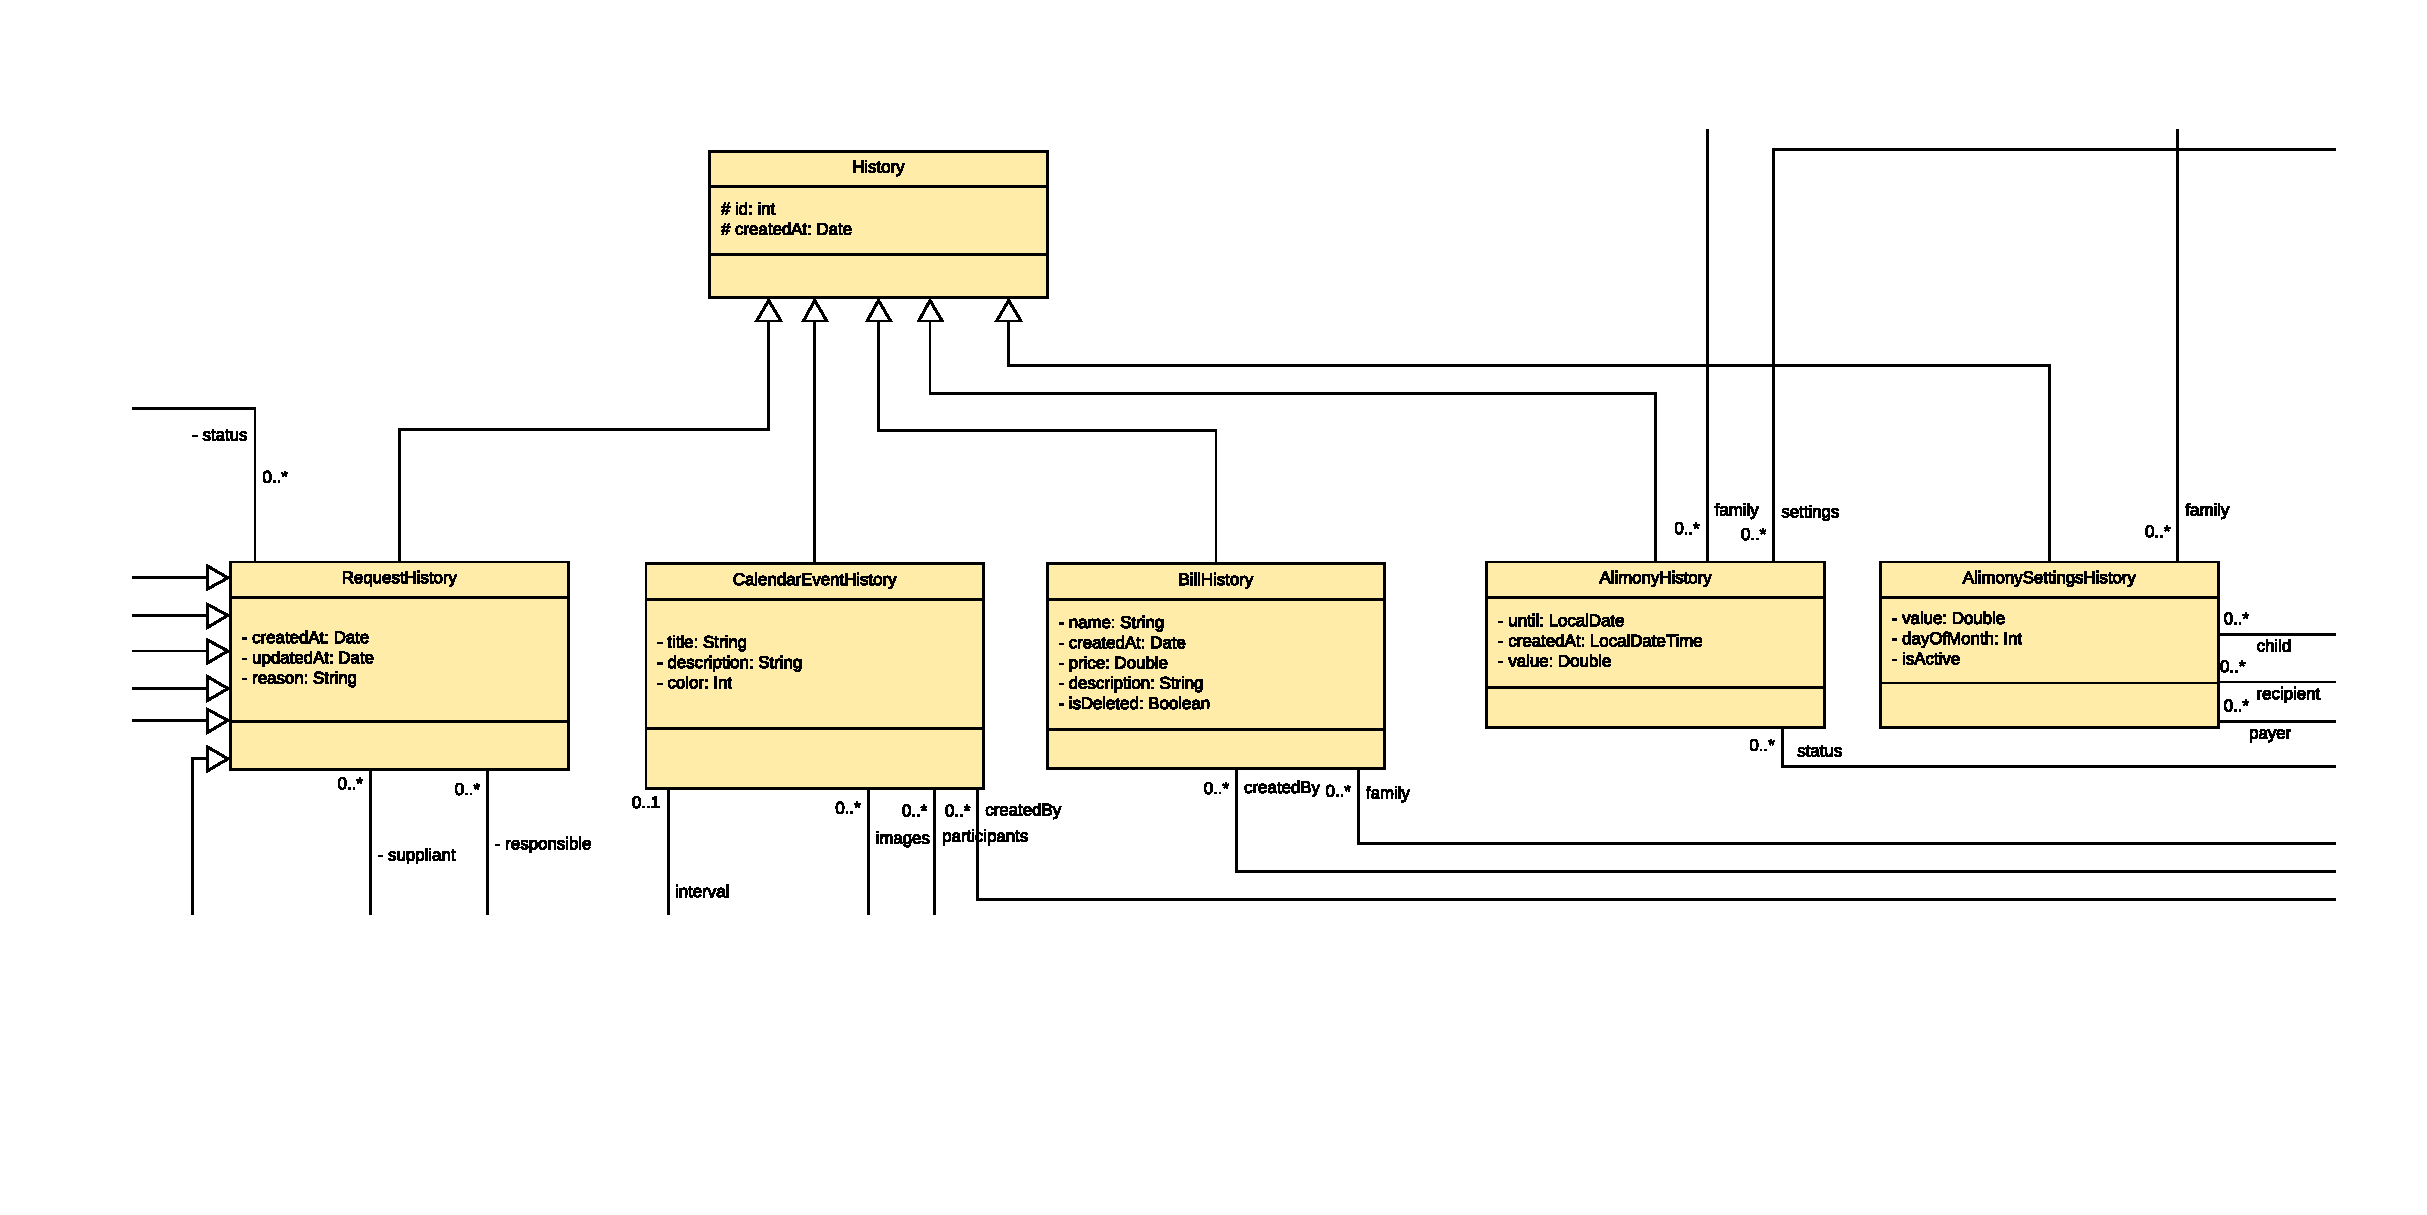
\includegraphics[width=1.0\textwidth]{pdfs/History1_2}
	        \caption[Návrh entity \texttt{History} po změnách návrhu]{Návrh entity \texttt{History} po navržení změn pro entity, kterým patří příslušné entity historie}\label{image:History1_2}
        \end{figure}
        Tato entita byla implementována jako poslední a všechny změny, které se ji týkají, jsou srozumitelné jenom po přečtení všech změn návrhu. Než se začít návrh vhodných změn této entity, byla potřeba nejdřív upravit návrh podle implementovaných změn v příslušných entitách (viz obrázek \ref{image:History1_2}).
        
        Dalším krokem úprav je navržení úprav, které už není nutné, ale výrazně zlepšují výsledný návrh programu:
        \begin{itemize}
            \item přidání do každé entity, reprezentující historii, odkazy na příslušné entity; Například, entita \texttt{AlimonyHistory} bude mít navíc odkaz na entitu \texttt{Alimony};
            \item zavedení nové entity \textit{CareDaysSettingHistory} podle návrhu entity \textit{CareDaysSetting}, která byla popsána v sekci \ref{navrh:upravy:caredays}.
        \end{itemize}
        %TODO image
        Výsledný návrh entity \verb|History| (viz přílohu \ref{dodatek:DomainModel2}) byl kompletně implementován. Také byly přidány řadiče pro každý typ historie, které poskytují možnost vyhledat záznamy. Uživatel nemůže vytvořit nový záznam historie nebo změnit již existující záznam. Proto API serveru nepodporuje příslušné požadavky. Vytvoření instancí historie se provádí serverem automaticky při aktualizacích příslušných entit.
        Spravování entit historie v doménové vrstvě bylo rozděleno do dvou logických bloků. První blok se zabývá spravováním požadavků Android aplikace. Každý typ historie má vlastní rozhraní reprezentující metody, které je možné provádět s touto entitou. Druhým logickým blokem je proces vytváření instancí historie. Za tímto účelem bylo přidané rozhraní \verb|InternalHistoryService|, které poskytuje metodu \verb|toHistory| pro uložení instance do databáze.
        Metoda očekává jako parametr instanci třídy před provedením změn a konvertuje utto instanci do příslušné instance historie. Každý typ historie také má vlastní konvertor z entity do entity historie. Například, po vložení do metody \verb|toHistory| parametru typu \verb|Bill|, bude zavolán konvertor \verb|BillToHistoryConvertor|, který vrátí instanci třídy \verb|BillHistory|. 

\section{Návrh bezpečnosti}\label{navrh:bezpecnost}
    \subsection{OAuth 2.0}
        % TODO
        Za účelem zabezpečení procesu autorizace byl zvolen protokol OAuth 2.0. Tento protokol je nativně podporován frameworkém Spring. Proto byla provedena jeho konfigurace, která vyžadovala implementaci následujících rozhraní:
        \begin{itemize}
            \item \texttt{UserDetailsService} -- pro definování zdroje informace o uživatelích;
            \item \texttt{WebSecurityConfigurerAdapter} -- pro definování implementaci rozhraní \texttt{UserDetailsService} a nastavení kontextu bezpečnosti;
            \item \texttt{AuthorizationServerConfigurerAdapter} -- pro nastavení procesu přihlašování;
            \item \texttt{ResourceServerConfigurerAdapter} -- pro nastavení přístupu do řadičů.
        \end{itemize}
        
        Rozhraní \verb|UserDetails| bylo implementováno pro každý profil zvlášť. Pro pohodlný proces vývoje byl přidán uživatel s rolí \enquote{ROLE\_ROOT} pro profil \verb|dev|. Za účelem testování byly přidány implicitní uživatele pro profil \verb|test|. Třetí implementace byla implementována pro profil produkce, proto žádného implicitního uživatele táto implementace nemá.
        
    \subsection{HTTPS}
        V předchozí implementaci aplikace byl použit protokol HTTP\footnote{\textit{Hypertext Transfer Protocol}}, který nezaručuje bezpečnou komunikaci mezi klientem a serverem. Proto tento protokol byl nahrazen protokolem HTTPS\footnote{\textit{Hypertext Transfer Protocol Secure}}, který vyžaduje podepsaný třetí stranou certifikát. Tento certifikát je uložen v aplikaci.
        
% \section{Návrh požadavků na změny}\label{navrh:requests}
%     Pro zaručení správného návrhu API je potřeba propojit výsledný návrh serverového backendu a Android aplikaci, která se řeší v rámci souběžné bakalářské práci. Proto v je potřeba v práci této bakalářské práci připravit API, které by bylo použitelné. Současný návrh Android aplikaci nepodporuje požadavky. Výsledná implementace API serveru také nepodporuje požadavky na změny za účelem vyvarování kolizí. V této 
\section{Profily}\label{navrh:profily}
    Během implementace serveru byla potřeba rozšířit návrh profilů aplikace. Původní návrh obsahoval jenom implicitní profil a profil vývoje, obsahující konfiguraci databáze H2. Výsledný návrh aplikace potřebuje více profilů, proto byly přidány dva další profily: profil pro produkci a profil pro testování. Příčinami přidání dalších profilů jsou rozdíly mezi konfiguracemi, která potřebují konkretní případy spouštěni aplikace. Princip chovaní profilu byl již zmíněn v sekci \ref{analyza:soucasnaImplementace:profily}, proto v této sekci budou popsáné provedené změny.
    
    Pro podrobnější popis přidaných profilu je potřeba nejdřív popsat výslednou konfigurací existujícího profilu, vytvořeného pro proces vývoje. Seznam provedených změn a rozšíření, které se navazují na tento profil:
    \begin{itemize}
            \item Rozšířena konfigurace databáze. Změny byly provedeny za účelem přesnější definice konfigurace (viz sekci \ref{navrh:db});
            \item Přidána nutná konfigurace pro bezpečnost aplikace, která byla popsána v sekci \ref{navrh:bezpecnost};
            \item Přidána proměnná do konfiguračního souboru, která zapíná pravidelné vytváření alimentů (viz sekci \ref{navrh:upravy:alimenty}) a také proměnná definující pravidlo, podle kterého se řídí plánováni spouštění této třídy;
            \item Přidána specifická implementace pro rozhraní \textit{UserDetails} (viz sekci \ref{navrh:bezpecnost});
            \item Přejmenován profil \enquote{development} na \enquote{dev}, za účelem lepší elegance kódu při definování několika profilu komponenty najednou.
    \end{itemize}
    
    Výše uvedena konfigurace je vhodná pro vývoj aplikace, ale zároveň není vhodná pro produkci a testování aplikace. Proto bylo rozhodnuto nechat v implicitním konfiguračním souboru jenom definici profilu, který by měla aplikace využit pro následující spuštění, a přidat další profily podle případů využití.
    
    Prvním profilem, který byl přidán, je profil pro produkci. Hlavním rozdílem tohoto profilu od profilu vývoje je použita databáze. Podrobněji zvolená databáze bude popsána v sekci \ref{navrh:db}. Pro tuto sekci je postačující zmínit, že zvolena databáze je PostrgesSQl. Druhou odlišností je jiná implementace rozhraní \verb|UserDetails|. Produkční verze aplikace by neměla mít \verb|root| uživatele. Jiný konfigurační soubor také dovoluje nechat konfiguraci pro produkci nedotčenou při možném velkém počtu změn v jiných profilech.
    Například, můžeme nechat vypnuté plánované vytváření alimentů pro vývojový profil.
    
    Druhým profilem, který byl přidán do aplikace, je profil pro testování. Změny se dotkly stejných aspektu jako i profilu produkce. Byla přidána nova implementace rozhraní \verb|UserDetails|, která obsahuje implicitních uživatele s různými rolemi. Také byla přidána konfigurace databáze. Pro tento profil byla zvolena stejná databáze jako i pro profil produkce. Takový postup zmenšuje šance na výskyt nečekaných chyb, působených použitím odlišné databáze v produkci.
    
\section{Databáze} \label{navrh:db}
    Použité databáze byly popsány v sekci \ref{resere:databaze}. V této sekci bude vysvětleno proč byly zvoleny tyto databáze.
    % Popis používané databáze už vyskytoval v rešerši (viz sekci \ref{resere:databaze}) a analýze (viz sekci \ref{analyza:soucasnaImplementace:databaze}), proto tady jenom zmíním, že se používá relační databáze H2. Pro popis zvolených databází pro proces realizace praktické části je potřeba zmínit, že aplikace byla rozdělena do různých profilů. Používána databáze je jedním z rozdílů těchto profilů. Podrobněji profily aplikace byly popsány v sekci \ref{navrh:profily} .
    
    Profil pro vývoj používá databázi H2. Stejná databáze byla použita při předchozí implementaci. Databáze nevyžadovala její nahrazeni jinou databází, protože nevyžaduje nastartování databázi zvlášť od aplikace, ale se nastartuje spolu s aplikací. Všechna data se ukládají přímo v paměti aplikace, proto po restartování aplikace smaže všechny vytvořené záznamy.
    % Zdroj databáze byl změněn z konkretního souboru na paměť aplikace, což znamená, že databáze se vytváří při každém spouštění aplikace a zničí se po její ukončení. Také byl definován konkretní dialekt databáze. Byl zvolen implicitní dialekt, který poskytuje databáze H2, protože zvolená databáze pro produkci.
    
    Pro profil produkce bylo rozhodnuto použit jinou databází. Byly zvoleny dva kandidáty: PostgresSQL a MySQL. Tyto databáze jsou jedeními z nepopulárnějších databázi na moment napsáni této bakalářské práci a zároveň jsou otevřeným softwarem. Po porovnání těchto dvou databázi, výslednou databází byla zvolena databáze PostgresSQL. Některá funkcionalita byla považovaná za důležitou i když není ještě využita v implementaci a návrhu. Příklady převah PostgresSQL nad MySQL: 
    \begin{itemize}
            \item PostgresSQL je objektově relační databáze\cite{postgres-about}, když MySQL je jenom relační databáze\cite{mysql-wiki}. Tohle znamená, že PostgresSQL dovoluje dědění tabulek a přetěžování metod;
            \item PostgresSQL poskytuje možnost definovat vlastní typy\cite{pstgres-create-type};
            \item autor této práce má zkušenosti s PostgresSQL.
    \end{itemize}
    Informace o rozdílech těchto databází byly převzaty s několika článku na internetu. Nejpoužitelnějšími pro autora této práce byly \cite{mysql-postgres1, mysql-postgres2}.
    
% \section{Implementace požadavků na změny}\label{impl:requests}
%     TODO requests
    
\section{Návrh testování}\label{navrh:testovani}
    % Pro testování kódu budou využity frameworky JUnit 5 a Spring. Podrobný popis těchto frameworků byl v sekci \ref{resere:testovani}. Testování se skládá s \texttt{unit}\footnote{testy, zaměřené na ověření správnosti fungování samostatně testovatelné části programu} testů a \texttt{integration}\footnote{testy, zaměřené na ověření správné komunikace mezi komponentami} testů. Návrh testů se bude podstatné lišit mezi sebou. Proto bude využita funkcionalita frameworku JUnit 5, který od verze 5 poskytuje možnost označovat testy pomocí tagů\cite{junit-tags}. Princip chování tagů najdete v sekci \ref{resere:testovani}. Podrobnější informaci o implementaci tagů bude popsána v sekci \ref{testovani:tagy}. Kompletní implementace testování bude popsána v kapitole \ref{testovani}.
    Pro testování kódu budou využity frameworky JUnit 5 a Spring. Tyto frameworky byly podrobně popsány v sekci \ref{resere:testovani}. Testování se skládá s \texttt{unit}\footnote{testy, zaměřené na ověření správnosti fungování samostatně testovatelných částí programu} testů a \texttt{integračních}\footnote{testy, zaměřené na ověření správné komunikace mezi komponentami} testů. Návrh testů se bude podstatné lišit mezi sebou. Proto bude využita funkcionalita frameworku JUnit 5, který od verze 5 poskytuje možnost označovat testy pomocí tagů\cite{junit-tags}. Podrobnější informaci o implementaci tagů bude uvedená v sekci \ref{testovani:tagy}. Kompletní implementace testování bude popsána v kapitole \ref{testovani}.
    
    \subsection{Unit testy}
        Unit testy využívají jenom funkcionalitu frameworku JUnit 5 a testují základní funkce. Otestovány mají byt třídy a metody, které mohou být otestovány samostatně. Také, tyto testy mají být označeny jako unit testy pomocí tagů.  %TODO popsat podrobneji
        
    \subsection{Integráční testy}
        Integrační testy budou testovat jednotlivé řadiče. Tyto testy jsou navrženy pomocí principu IoC. Tyto. testy také budou označeny jako integrační testy a zároveň jako pomalé testy.
        %C\footnote{princip, za kterého kontrola nad vytvořením a provázáním tříd vlastní framework}